% ============================================================
% Lecture 18 -- Computation of least square estimates in R
% ============================================================
\section{Computation of Least Squares Estimates in R}\label{sec:L18}

\lectureheader{18}{4gwbWg_Gq-4}{Week-5 R code \texttt{Feb21.r} (Boston lab: \texttt{names}, \texttt{coef}, \texttt{confint}, \texttt{predict}, diagnostic plots, \texttt{hatvalues}; Monte Carlo simulation; non-central $t$). The Week-5 lecture PDF was \emph{not} accessed.}

\begin{guiding*}
By the end of this lecture you should be able to:
\begin{itemize}
  \item extract every component of a fitted linear model in R and in Python;
  \item distinguish a confidence interval for the mean response from a prediction interval for a new response, and derive both;
  \item produce and interpret the four standard diagnostic plots;
  \item compute leverages (hat values) and identify high-leverage points;
  \item run a simple Monte Carlo simulation.
\end{itemize}
\end{guiding*}

\subsection{Recap}
The previous three lectures gave the estimates (\cref{sec:L15}), their standard errors, intervals and tests
(\cref{sec:L16}), and overall measures of fit (\cref{sec:L17}). This lecture walks through the rest of the R
code, which uses these results in practice on the \texttt{Boston} data.

\subsection{Inside a fitted model}
\texttt{names(lm.fit)} lists the stored components: \texttt{coefficients}, \texttt{residuals},
\texttt{fitted.values}, \texttt{rank}, \texttt{df.residual}, the QR decomposition, and others. \texttt{coef(lm.fit)} returns
$(34.5538,-0.9500)$ and \texttt{confint(lm.fit)} the intervals of \cref{ex:L16-boston}.

\begin{note}[How R actually solves the normal equations]
\texttt{lm} does not form $X\T X$. It computes a QR decomposition $X=QR$, where $Q$ ($n\times p$) has orthonormal columns
and $R$ ($p\times p$) is upper triangular. Then $X\T X\beta=X\T Y$ becomes $R\T R\beta=R\T Q\T Y$, i.e.\ $R\beta=Q\T Y$,
which is solved by back-substitution. This is numerically more stable, because the condition number of $X\T X$ is the
square of that of $X$. It also gives $\PX=QQ\T$ directly: $Q$ is an orthonormal basis of $\colsp{X}$, as in
\cref{lem:L14-projection}. \texttt{statsmodels} uses the Moore--Penrose pseudo-inverse by default, or QR with
\texttt{method="qr"}.
\end{note}

\subsection{Confidence and prediction intervals}
\texttt{predict(lm.fit, data.frame(lstat = c(5,10,15)), interval = "confidence")} and
\texttt{interval = "prediction"} give two different kinds of interval. At a new value $x_0$, let
$\hat Y_0=\hat\beta_0+\hat\beta_1x_0$ and $h_0=\frac1n+\frac{(x_0-\bar x)^2}{S_{xx}}$.

\begin{proposition}\label{prop:L18-intervals}
Assume normal errors in simple linear regression, and let $Y_0=\beta_0+\beta_1x_0+\eps_0$ be a new observation with
$\eps_0\sim\N(0,\sigma^2)$ independent of the data.
\begin{enumerate}
  \item $\hat Y_0\pm t_{n-2,1-\alpha/2}\,s\sqrt{h_0}$ is a $100(1-\alpha)\%$ \vocab{confidence interval} for the mean response $\beta_0+\beta_1x_0$.
  \item $\hat Y_0\pm t_{n-2,1-\alpha/2}\,s\sqrt{1+h_0}$ is a $100(1-\alpha)\%$ \vocab{prediction interval} for $Y_0$.
\end{enumerate}
\end{proposition}
\begin{proof}
$\hat Y_0=\lambda\T\hat\beta$ with $\lambda=(1,x_0)\T$. It is normal with mean $\beta_0+\beta_1x_0$ and variance
$\sigma^2\lambda\T(X\T X)^{-1}\lambda=\sigma^2h_0$ (\cref{prob:L15-3}). It is independent of $s^2$ (\cref{thm:L16-dist}).
(1) Then $(\hat Y_0-\beta_0-\beta_1x_0)/(s\sqrt{h_0})\sim t_{n-2}$, exactly as in the proof of \cref{thm:L16-dist}(4).
(2) $Y_0-\hat Y_0$ has mean $0$ and, since $\eps_0$ is independent of $\hat Y_0$, variance $\sigma^2+\sigma^2h_0$. It is
normal, and it is independent of $s^2$, because $\eps_0$ is independent of all the data. Hence
$(Y_0-\hat Y_0)/(s\sqrt{1+h_0})\sim t_{n-2}$, and the interval follows as in \cref{cor:L16-ci}.
\end{proof}
The confidence interval reflects only the uncertainty in the fitted line. It shrinks to zero width as
$n\to\infty$. The prediction interval also contains the irreducible noise $\eps_0$ of a new observation, so it never
becomes narrower than about $\pm1.96\sigma$.

\begin{example}[Boston]\label{ex:L18-predict}
With $n=506$, $s=6.2158$ and $t_{504,0.975}=1.9647$:
\begin{center}
\begin{tabular}{cccc}\hline
\texttt{lstat} & fit & 95\% confidence interval & 95\% prediction interval\\\hline
5 & 29.8036 & (29.0074, 30.5998) & (17.5657, 42.0415)\\
10 & 25.0533 & (24.4741, 25.6326) & (12.8276, 37.2791)\\
15 & 20.3031 & (19.7316, 20.8746) & (8.0777, 32.5285)\\\hline
\end{tabular}
\end{center}
Both intervals are centred at the same fitted value. The prediction intervals are about $20$ times wider.
\end{example}

\begin{example}[By hand]\label{ex:L18-hand}
For the four-point data at $x_0=5$: $\hat Y_0=0.5+1.4\times5=7.5$ and
$h_0=\frac14+\frac{(5-2.5)^2}{5}=1.5$ (an extrapolation, so $h_0$ is large). With $s^2=0.1$ and $t_{2,0.975}=4.3027$:
the confidence interval is $7.5\pm4.3027\sqrt{0.15}=7.5\pm1.6664=(5.8336,\,9.1664)$, and the prediction interval is
$7.5\pm4.3027\sqrt{0.25}=7.5\pm2.1514=(5.3487,\,9.6514)$.
\end{example}

\subsection{Diagnostic plots and leverage}
\texttt{par(mfrow=c(2,2)); plot(lm.fit)} draws four diagnostic plots: residuals against fitted values, a normal
Q--Q plot, a scale--location plot, and residuals against leverage. The code then draws
\texttt{plot(predict(lm.fit), residuals(lm.fit))} and \texttt{plot(predict(lm.fit), rstudent(lm.fit))}.
For Boston, the residuals against fitted values form a clear U-shape (\cref{fig:L18-diag}). This is evidence of
\emph{non-linearity}, exactly as in Forbes' data (\cref{sec:L06}). ISLR's lab later adds a term
$\texttt{lstat}^2$.

\begin{definition}[Leverage]\label{def:L18-leverage}
The \vocab{leverage} (hat value) of observation $i$ is $h_{ii}=(\PX)_{ii}$, the $i$th diagonal entry of the hat matrix.
The name comes from $\hat Y=\PX Y$: the projection matrix ``puts the hat on $Y$''. The
\vocab{studentized residual} (R: \texttt{rstudent}) is $\hat e_i/(s_{(i)}\sqrt{1-h_{ii}})$, where $s_{(i)}$ is the RSE of
the fit without observation $i$.
\end{definition}

\begin{proposition}\label{prop:L18-hat}
(1) $0\le h_{ii}\le1$ and $\sum_ih_{ii}=\rank X$. (2) $\Var(\hat e_i)=\sigma^2(1-h_{ii})$. (3) In simple linear regression
$h_{ii}=\frac1n+\frac{(x_i-\bar x)^2}{S_{xx}}$.
\end{proposition}
\begin{proof}
(1) Since $\PX$ is symmetric and idempotent, $h_{ii}=(\PX^2)_{ii}=\sum_l(\PX)_{il}^2=h_{ii}^2+\sum_{l\ne i}(\PX)_{il}^2\ge h_{ii}^2$. So
$h_{ii}\ge h_{ii}^2$, which gives $0\le h_{ii}\le1$. Also $\sum_ih_{ii}=\tr\PX=\rank X$ (\cref{lem:L14-projection}).
(2) $\hat e=(I-\PX)Y$, so $\Cov(\hat e)=\sigma^2(I-\PX)(I-\PX)\T=\sigma^2(I-\PX)$. Its $i$th diagonal entry is $\sigma^2(1-h_{ii})$.
(3) $h_{ii}=x_i\T(X\T X)^{-1}x_i$ with $x_i=(1,x_i)\T$. Using the inverse in the proof of \cref{cor:L15-slr},
$h_{ii}=\frac{\sum_lx_l^2-2x_i\sum_lx_l+nx_i^2}{nS_{xx}}=\frac{S_{xx}+n(x_i-\bar x)^2}{nS_{xx}}$. This is the stated formula, since
$\sum_lx_l^2-2x_i n\bar x+nx_i^2=S_{xx}+n\bar x^2-2nx_i\bar x+nx_i^2$.
\end{proof}
A point with large leverage has an $x$-value far from $\bar x$. It can pull the fitted line towards itself. For Boston,
\texttt{which.max(hatvalues(lm.fit))} returns observation $375$, which has the largest \texttt{lstat} ($37.97$) and
$h_{375,375}=0.02687$. The average leverage is $p/n=2/506=0.00395$, and the hat values sum to exactly $2$.

\begin{figure}[ht]
\centering
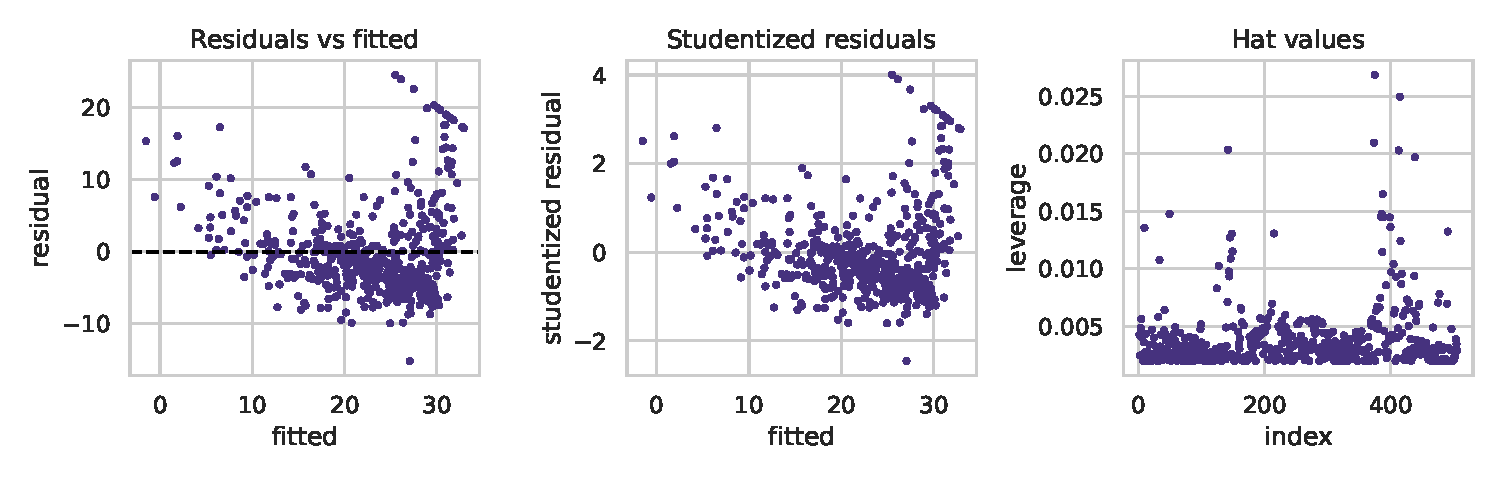
\includegraphics[width=\textwidth]{figures/L18_boston_diag.pdf}
\caption{Boston: residuals and studentized residuals against fitted values (note the curvature), and hat values
by observation index (the maximum is at observation 375).}
\label{fig:L18-diag}
\end{figure}

\subsection{A Monte Carlo simulation}
The code ends with a simulation:
\begin{center}
\begin{minipage}{0.8\textwidth}\small\ttfamily
OneFourthPiSamples = replicate(100, \{ u <- runif(10000); v <- runif(10000);\\
\quad z <- sqrt(u\textasciicircum2 + v\textasciicircum2); sum(z < 1)/10000 \})
\end{minipage}
\end{center}
A point $(U,V)$ uniform on the unit square falls inside the quarter disc $\{u^2+v^2<1\}$ with probability equal to its area,
$\pi/4=0.7854$. Each replicate estimates $\pi/4$ by the proportion of $10\,000$ points inside, with standard error
$\sqrt{(\pi/4)(1-\pi/4)/10000}=0.0041$. With the notebook's seed the $100$ replicates have mean $0.7858$ and
standard deviation $0.0047$. The same idea, repeat an experiment and look at the distribution of an estimate, is how the
notebooks check sampling distributions such as those of \cref{thm:L16-dist}. The instructor uses it for least squares
estimators in Week~7.

\subsection{Computation}
\begin{center}\small
\begin{tabular}{@{}>{\raggedright\arraybackslash}p{7cm}>{\raggedright\arraybackslash}p{8.4cm}@{}}\hline
R & Python (\texttt{statsmodels})\\\hline
\texttt{names(lm.fit)}, \texttt{coef}, \texttt{confint} & \texttt{dir(fit)}, \texttt{fit.params}, \texttt{fit.conf\_int()}\\
\texttt{predict(..., interval="confidence")} & \texttt{fit.get\_prediction(new).summary\_frame()} (\texttt{mean\_ci\_*})\\
\texttt{predict(..., interval="prediction")} & same frame, columns \texttt{obs\_ci\_*}\\
\texttt{plot(lm.fit)} & residual, Q--Q (\texttt{sm.qqplot}), leverage plots\\
\texttt{hatvalues}, \texttt{rstudent} & \texttt{fit.get\_influence().hat\_matrix\_diag}, \texttt{.resid\_studentized\_external}\\
\texttt{replicate(100, \{...\})} & list comprehension with \texttt{rng.uniform}\\\hline
\end{tabular}
\end{center}
See \nb{week05/L18\_computation\_in\_R.ipynb}.

\subsection{Summary}
\begin{itemize}
  \item At $x_0$: confidence interval $\hat Y_0\pm t\,s\sqrt{h_0}$ for the mean, prediction interval $\hat Y_0\pm t\,s\sqrt{1+h_0}$ for a new $Y$, where $h_0=\frac1n+\frac{(x_0-\bar x)^2}{S_{xx}}$.
  \item Leverage $h_{ii}=(\PX)_{ii}\in[0,1]$, $\sum h_{ii}=p$, $\Var\hat e_i=\sigma^2(1-h_{ii})$.
  \item Boston: the residuals show curvature, and the highest leverage is observation $375$.
  \item Monte Carlo: repeat, then summarise the estimates.
\end{itemize}

\subsection{Exercises}
\begin{problem}\label{prob:L18-1}
Show that the prediction interval at $x_0=\bar x$ has half-width $t_{n-2,1-\alpha/2}\,s\sqrt{1+1/n}$.
\end{problem}
\begin{problem}\label{prob:L18-2}
For the four-point data compute all four hat values and check that they sum to $2$.
\end{problem}
\begin{problem}\label{prob:L18-3}
Fit \texttt{medv \textasciitilde\ lstat + I(lstat\textasciicircum2)} and compare $R^2$ and the residual plot with the straight-line fit.
\end{problem}
\begin{problem}\label{prob:L18-4}
Estimate $\pi$ by Monte Carlo with $10^6$ points. How many points are needed for the standard error of the estimate of $\pi$ to be below $0.001$?
\end{problem}

\subsection{Further reading}
ISLR \S3.1--3.3 and Lab~3.6; Weisberg, \emph{ALR}, Chapter~9 (regression diagnostics); Christensen, Chapter~12.
